
\chapter{Einleitung}

\section{Motivation}
Der Begriff \enquote{autonomes Fahren} hat spätestens seit den Tesla Autos einen allgemeinen Bekanntheitsgrad erreicht. Um ein Auto selbstständig fahren lassen zu können, müssen erst viele Hürden gemeistert werden, zum Beispiel das Spur halten, auch bei fehlenden Fahrspurmarkierungen, das Interpretieren von Stoppschildern und navigieren durch komplexen Kreuzungen. \todo{ref tesla.com?}

Bevor das Auto Entscheidungen treffen kann, muss es zuallererst ein Modell seines Umfelds erstellen oder zur Verfügung gestellt bekommen. Aber vielleicht kann ein Auto nicht immer selbständig genügend Informationen zu seinem Umfeld sammeln? \todo{(huhuhu Server implied huhuhu)}
%Diese Arbeit beschäftigt sich mit genau dem Thema, einem selbst fahrendem Auto Informationen zu anderen Teilnehmern an einer Kreuzung zu vermitteln.
\todo{fix 404}

\section{Projektkontext}
\begin{figure}[H]
	\label{test 123}
	\centering
	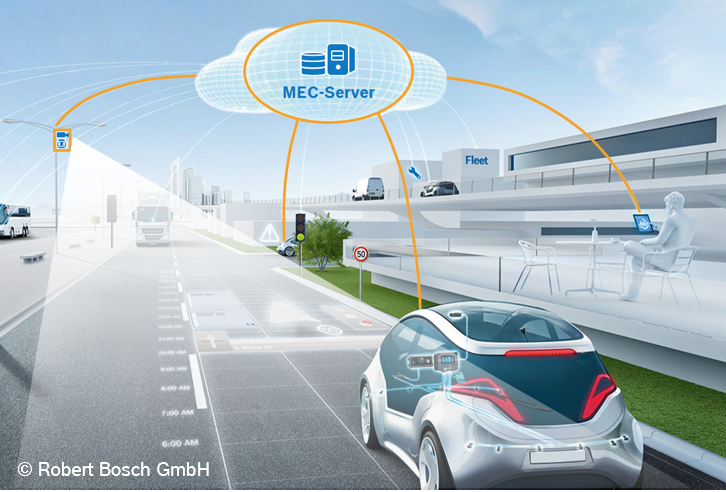
\includegraphics[width=\textwidth]{images/MECView_Schaubild_BoschStyle_V2.png}
	\caption{MEC-View Schaubild der Robert Bosch GmbH \cite{mec:home} {}}
	\captionsource{\url{https://www.uni-due.de/~hp0309/images/Schaubild_BoschStyle_V2.png}}
\end{figure}

Diese Abschlussarbeit befasst sich mit dem \gls{mec}-Server, der Teil des \gls{mec}-View Forschungsprojekt ist.
Das \gls{mec}-View Projekt wird durch das \gls{bmwi} gefördert und befasst sich mit der Thematik autonom fahrender Fahrzeuge.
Es soll erforscht werden ob und in wie weit eine durch externe Sensorik geleistete Unterstützung nötig und möglich ist um in eine Vorfahrtsstraße autonom einzufahren.

Das Forschungsprojekt ist dabei ein Zusammenschluss verschiedener Unternehmen:
\begin{center}
	\begin{tabular}{l|l}		
		Unternehmen & Aufgabenbereich \\ \hline \hline
		Bosch & Hochautomatisiertes Fahrzeug \\
		Osram & \glqq{}Intelligente\grqq{} Infrastruktursensoren \\ 
		Nokia & 5G Mobilfunk, Mobile Edge Computing (MEC) \\
		Universität Ulm & Sensordatenfusion, Prädiktion \\
		\rowcolor{lightgray!20} IT-Designers Gruppe & MEC-Server Architektur\\
		\rowcolor{lightgray!20} & Mikroskopische Verkehrsanalyse \\
		\rowcolor{lightgray!20} & Verhaltensanalyse \\
		TomTom & Hochgenaue statische und dynamische Karten \\
		Daimler & Fahrstrategien \\
		& Verhaltensanalyse \\
		& Streckenfreigabe \\
		Universität Duisburg & Mikroskopisch, stochastische Simulationsmodelle
	\end{tabular}
\end{center}


\subsection{Ablauf}
Externe Sensoren übermitteln erkannte Fahrzeuge via Mobilfunk an einen \gls{mec}-Server, der direkt am Empfängerfunkmast angeschlossen ist. \todo{platform, vm?}
Nachdem die erkannten Fahrzeuge der verschiedenen Sensoren zusammengeführt wurden (Fusions-Algorithmus), sollen sie an das autonom fahrende Fahrzeug über Mobilfunk übermittelt werden.
Somit erhält das Fahrzeug bereits im Voraus Einsicht über eventuelle Möglichkeiten in die Vorfahrtsstraße einzufahren und könnte deshalb beispielsweise die Geschwindigkeit anpassen.
Zudem sollen bei unübersichtlichen Kreuzungen somit zuverlässiger andere Verkehrsteilnehmer erkannt werden.

\subsection{Sicherheit}
\todo{überhaupt relevant?}
Da bei Fehlern möglicherweise andere Verkehrsteilnehmer zu Schaden kommen können, müssen diverse Sicherheitsrichtlinien beachtet werden. Die Industrienorm ISO 26262 beschreibt dabei verschiedene Vorgehensweisen,
unter anderem eine \gls{fba}, Risikoabschätzung durch Einstufung nach \glspl{sil} und beschreibt Gegenmaßnahmen.


\section{Zielsetzung}

Das Ziel ist es, eine alternative Implementierung des \gls{mec}-View Servers in Rust zu schaffen.
Durch die Garantien (\autoref{rust:guarantees}) von Rust wird erhofft, dass der menschliche Faktor als Fehlerquelle gemindert wird und somit eine fehlertolerantere und sicherere Implementation geschaffen werden kann.

\todo{?} Für eine bessere Wartbarkeit und Nachvollziehbarkeit soll die Implementation in Ihrer \todo{Struktur/}Architektur der C++ Implementation ähneln.


\section{Aufbau der Arbeit}

Diese Arbeit ist im wesentlichen in die folgenden Themengebiete aufgeteilt: Grundlagen, Anforderungs- und Systemanalyse, Systementwurf und Implementation und Auswertung.

Im Themengebiet Grundlagen sollen wesentliche Bestandteile dieser Arbeit erläutert und erklärt werden.
Hierzu zählt zum einen die Programmiersprache Rust in ihrer Entstehungsgeschichte \todo{ref}, Garantien \todo{ref}  und Sprachfeatures \todo{ref}, zum anderen die hochperformante, serverbasierte Kommunikationsplattform mit ihren Protokollen \todo{ref} und dem Systemkontext in dem diese betrieben wird.

In der Anforderungs- und Systemanalyse wird der Kontext in dem das System betrieben werden soll genauer betrachtet. Umzusetzende funktionale und nicht-funktionale Anforderungen werden aufgestellt sowie eine Übersicht von Systemen mit denen interagiert wird.

Das Themengebiet Systementwurf und Implementation befasst sich mit dem theoretischen und praktischen Lösen der im vorherigen Kapitel aufgestellten Anforderungen. Aufgrund der Tatsache, dass es sich hierbei
um eine alternative Implementation handelt, wird zur bestehenden C++ Implementation Bezug genommen.
Auf architektonische Unterschiede im Systementwurf, die sich aufgrund von Sprach- und Bibliotheksunterschiede, werden hier genauer beschrieben.

Zuletzt wird eine Auswertung der Implementation aufgezeigt. \todo{michael.write\_more();}